%%%%%%%%%%%%%%%%%%%%%%% file typeinst.tex %%%%%%%%%%%%%%%%%%%%%%%%%
%
% This is the LaTeX source for the instructions to authors using
% the LaTeX document class 'llncs.cls' for contributions to
% the Lecture Notes in Computer Sciences series.
% http://www.springer.com/lncs       Springer Heidelberg 2006/05/04
%
% It may be used as a template for your own input - copy it
% to a new file with a new name and use it as the basis
% for your article.
%
% NB: the document class 'llncs' has its own and detailed documentation, see
% ftp://ftp.springer.de/data/pubftp/pub/tex/latex/llncs/latex2e/llncsdoc.pdf
%
%%%%%%%%%%%%%%%%%%%%%%%%%%%%%%%%%%%%%%%%%%%%%%%%%%%%%%%%%%%%%%%%%%%


\documentclass[runningheads,a4paper]{llncs2e/llncs}

\usepackage{amssymb}
\setcounter{tocdepth}{3}
\usepackage{graphicx}
\usepackage{amsmath}
\usepackage{todonotes}

\usepackage{url}
\newcommand{\keywords}[1]{\par\addvspace\baselineskip
\noindent\keywordname\enspace\ignorespaces#1}

\begin{document}

\mainmatter  % start of an individual contribution

% first the title is needed
%\title{Using locality properties to improve distributed algorithm}
\title{Locality-aware Cooperation in Distributed IaaS Infrastructures}

% the name(s) of the author(s) follow(s) next
%
% NB: Chinese authors should write their first names(s) in front of
% their surnames. This ensures that the names appear correctly in
% the running heads and the author index.
%
\author{Jonathan Pastor\inst{1}, Marin Bertier\inst{2}, Flavien Quesnel\inst{1},
Adrien Lebre\inst{1} \and Cedric Tedeschi\inst{3}}
%
%\authorrunning{Lecture Notes in Computer Science: Authors' Instructions}
% (feature abused for this document to repeat the title also on left hand pages)

% the affiliations are given next; don't give your e-mail address unless you
% accept that it will be published
\institute{ASCOLA Research Group,
Mines Nantes / Inria / LINA, Nantes, France\\ 
\email{firstname.lastname@mines-nantes.fr} 
\and ASAP Research Group, INSA / Inria / IRISA, Rennes, France\\
\email{marin.bertier@irisa.fr} 
\and Myriads Research Group, Universit\'{e} de Rennes 1 / Inria / IRISA, Rennes,
France\\
\email{cedric.tedeschi@inria.fr} }

\maketitle

    Most current infrastructures for cloud computing leverage static
    and greedy policies for the placement of virtual machines. Such
    policies impede the optimal allocation of resources and the
    satisfaction of operational guarantees like service-level
    agreements. In recent years, more dynamic and often more efficient
    policies based, \eg on consolidation and load balancing
    techniques, have been developed and investigated. New policies are
    typically evaluated either using testbeds or \emph{in-vivo}
    experiments. However, due to the underlying complexity of cloud
    infrastructures, testbeds typically have to be tailored to
    specific restricted configurations and experiments on real
    infrastructures are necessarily of limited scale.

    In this article, we propose \vmps, a dedicated simulation
    framework to perform in-depth investigations of VM placement
    algorithms and compare them in a fair way. This framework, built
    on top of the \sg simulation platform, notably provides
    programming support to easy the implementation of placement
    algorithms and runtime support dedicated to load injection and
    execution trace analysis. \vmps supports the simulation of a large
    set of real-world configurations, while allowing researchers to
    conduct experiments at large scales. We also report on a
    validation of our framework by implementing and investigating
    representative algorithms for three classes of placement
    algorithms: centralized, hierarchical and fully-distributed ones.


\section{Introduction}

%%%
\subsection{DVMS}\label{ssec:dvms}

%\subsubsection{Overview.}
DVMS~\cite{quesnel:ispa2013,quesnel:cpe2012} (Distributed Virtual Machine Scheduler) is a
framework that schedules VMs cooperatively and dynamically in large-scale distributed
systems. It is deployed as a set of agents that are organized following a ring topology
and that cooperate with one another to guarantee that VM demands are satisfied during
their executions. Concretely, when a node \footnote{In the following, 
\emph{node} and \emph{PM} will refer to the same entity (\emph{i.e} physical 
server of the infrastructure).} cannot guarantee the QoS for its hosted VMs or
when it is under-utilized, it starts an iterative scheduling procedure~(ISP) by querying
its first neighbor to find a better placement; it thus becomes the initiator of the ISP.
If the neighbor cannot satisfy the request, it is forwarded to the following free
node until the ISP succeeds. When a viable mapping has been found, the leader (\ie the last
peer that has taken part to the ISP) reconfigures the system by performing adequate VM
migrations. Such an approach allows each ISP to send requests only to a minimal number of
nodes and even though an ISP can reserve all nodes if the corresponding problem is
particularly hard to solve (thus guaranteeing that a solution will always be found if it
exits), experiments have shown that in most cases ISPs involve only few
nodes. Moreover, the DVMS proposal allows several ISPs to occur independently at the same
moment throughout the infrastructure; in other words, scheduling is performed on
partitions of the system that are created dynamically, which significantly improves the
reactivity of the system. To prevent conflicts that could occur if several ISPs performed
concurrent operations on the same PMs or VMs, it should be emphasized that PMs are reserved for
exclusive use by a single ISP.

An example involving three partitions is shown in Figure~\ref{fig:isp}; in particular, we
can see the growth of partition~1 between two steps. Explaining in detail the notion of
``first out'' is beyond the scope of this article but readers can consider that the
``first out'' relation enables to handle communications efficiently, as each node involved
in a partition can forward a request directly to the first node on the outside of its
partition~\cite{quesnel:cpe2012}.

\begin{figure}[h!]
  \centering
  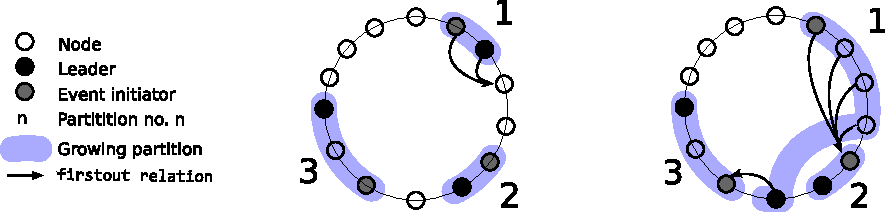
\includegraphics[width=0.9\linewidth]{Figures/resourceAcquisition-standard.pdf}
  \caption{Solving three problems simultaneously and independently with DVMS.}%
\small{The ring has been matched on top of three distinct clusters.}
  \label{fig:isp}%
\vspace*{-.3cm}
\end{figure}

We formally proved the correctness of DVMS using temporal logic, and we validated the first version of the prototype
at large scale (by means of simulations involving up to 80k VMs and 8k nodes and with experiments on the Grid'5000 testbed involving
up to 4.7k VMs and 470 nodes~\cite{quesnel:ispa2013}).

As discussed earlier, one limitation of this approach is related to its ring topology that
prevents it from taking into account the actual network topology.
%\subsubsection{Limitations of The Ring}
%
%Even though  DVMS can be deployed across several sites, it performs better on a
%cluster.
%
%The reason is simple.
%
%The ring is built without taking account of the network  topology; 
In other words, if the ISP strategy enables to limit the size of one partition to a
minimal number of nodes, these nodes are selected without considering the network
conditions at the time the ISP starts. This can lead to inefficient situations where VM
migrations occur between two nodes that are far from each other, which lasts longer than a
migration between two close nodes. Obviously the ring can be built to limit the
distance between peers globally (\ie peers of the same region/area would be grouped
together as illustrated in Figure~\ref{fig:isp}). However, in such a case, at least two
nodes of each group are directly connected to two far nodes.
%
Note that an approach such as the one proposed in~\cite{superchord}, which consists in
deploying one ring per site and relying on a \emph{super-ring}
to interconnect few representatives of each local ring, would not solve many
problems. Besides problems inherent to hierarchical and structured overlay networks, this
solution would not provide a good answer to locality: When going out of the local ring, it
would still not be possible to find the next closest ring.
%
%To sum up, the DVMS proposal lacks of a topology that can consider locality
%properties of a multi-sites infrastructure. 

% Autres limitations :
% -absence de tolerance aux pannes
% -peu d'evenements geres (surcharge d'un noeud)
% -ne prend pas en compte les liens entre VMS

\subsection{Overlay Networks and Locality}

As illustrated in the previous paragraph, one of the primary downsides of overlay networks
lies in that they break the physical topology by connecting nodes that have no physical
proximity.
%
Besides hierarchical attempts in building locality-aware overlay
networks~\cite{superchord,XuMK03,ECAN}, we can first mention the locality
improvement mechanisms of the Pastry structured overlay
network~\cite{pastry}. In order to reduce the latency of the routing process,
each node is given the opportunity to choose the closest nodes to fill its
routing table. Learning the existence of new nodes relies on a periodic exchange
of parts of routing tables.

Similar mechanisms have been adopted within unstructured overlay networks to make their
logical connections reflect the physical proximity of nodes, each node discovering its
closest nodes through gossiping. Note that the proximity between two nodes can be
estimated through any transitive metric, in particular the latency between the
nodes~\cite{tman}.

These approaches need to constantly maintain the knowledge of close nodes in order to
provide the \emph{best} node possible at the cost of periodic communications (uncorrelated
to the actual amount of requests to be processed by the overlay network).

The overlay network we propose in this paper differs in that it adopts a lazy approach consisting
in searching close nodes only upon receipt of requests. This way, the quality of the response
is proportional to the frequency of requests.

Our protocol relies on the Vivaldi protocol~\cite{dabek:2001:sigcomm04} to detect close
nodes. Vivaldi places nodes in a multi-dimensional space. Each node is given coordinates
inside this space reflecting its physical location. The protocol is based on simple
message exchanges. Initially, each node is given a random position in the space and
chooses (possibly arbitrarily) a small subset of nodes, composing its \emph{view}. Then,
each node starts estimating the round trip time between itself and another node chosen
randomly in its view, and adapts its distance with this node in the space accordingly,
coming closer to it or moving away from it. The nodes can repeat this step
independently (each with another node from its view), to improve the accuracy of the
positioning. A globally accurate positioning of nodes can be obtained very quickly (in a
small number of such steps) if nodes have a few long-distance nodes in their view and if the
network is not excessively dynamic. These long distance links can be easily maintained.

Recall that Vivaldi does not allow to directly know the nodes that are close in
the network, but to be able to recognize them through their coordinates. Our
overlay relies on the examination of Vivaldi coordinates of nodes discovered
during the processing of requests sent to it.










\subsection{Locality-aware  overlay network}

\CT{Vivaldi + spirale}

We here present our lazy locality-aware overlay network which underlies the VM
scheduling platform we developed. It is made of two layers. The lower layer
strongly rely on the Vivaldi protocol to make nodes aware of their position in
the platform. The higher layer takes its roots in the classic Dijkstra's
shortest parth algorithm to collect a set of close nodes starting from a given
position.

\CT{The remaining of the section is based on the book chapter.}

\subsubsection*{Giving a position to nodes}

The initial configuration of the physical network can take an arbitrary
shape. As already mentioned, Vivaldi~\cite{dabek:2001:sigcomm04} is a
distributed protocol assigning coordinates in the plane to nodes of a
distributed set of nodes. Each node is equipped with a \emph{view} of the
network, \emph{i.e.}, a set of nodes it knows. Coordinates obtained by a node
reflects its \emph{position} in the network, \emph{i.e.}, close nodes in the
network are given close coordinates in the plane. To achieve this, each node
checks the round trip time between itself and another node (randomly chosen
among nodes in its view) and adapts its distance (by changing its coordinates)
with this node in the plane accordingly. % See Figure~\ref{fig:vivaldi_before} and
% Figure~\ref{fig:vivaldi_after} for an illustration of 4 nodes~(A, B, C and D)
% moving according to the Vivaldi protocol.
A globally accurate positioning of nodes can be
obtained if nodes have a few long-distance nodes in their
view~\cite{dabek:2001:sigcomm04}. These long distance links can be easily
maintained by means of a simple gossip protocol.

% \begin{figure}[!b]
% 	\vspace*{-.3cm}
%   \begin{minipage}[c]{.45\linewidth}
%    \hspace*{-0.5cm}
%       	\centering 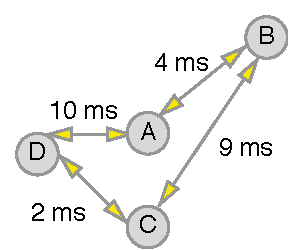
\includegraphics[width=3.4cm]{./FIGS/vivaldi_before.pdf}

%    \hspace*{0.5cm}
% 		\caption{Vivaldi plot before updating positions. Each node pings other nodes. Each node maintains a map of distance.}
% \label{fig:vivaldi_before}
%    \end{minipage}
% \hspace*{0.6cm}
%    \begin{minipage}[c]{.45\linewidth}
%    	\centering 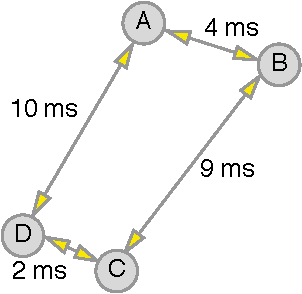
\includegraphics[width=3.4cm]{./FIGS/vivaldi_after.pdf}
% 		\caption{Vivaldi plot after updating positions. The computed
%                   positions of other nodes have been updated.}
% 		\label{fig:vivaldi_after} 
%   \end{minipage} \hfill
% \end{figure}

\subsubsection*{Searching for Close Nodes}

Once the map is achieved (each node knows its coordinates), we are able to
decide whether two nodes are \emph{close} by calculating their
distance. However, the view of each node does not \emph{a priori} contain its
closest nodes. Therefore, we need additional mechanisms to locate a set of nodes
that are close to a given initial node -- Vivaldi gives a \emph{location} to
each node, not a neighborhood. We use a modified distributed version of the
classic Dijkstra's shortest path algorithm. The goal is to build a
\emph{spiral}\footnote{The term \emph{spiral} is here a misuse of language,
since the graph actually drawn in the plane might contain crossing edges.}
interconnecting the nodes in the plane that are the closest ones to a given
initial node.

Let us consider that our initial point is a node called $I$. The first step is
to find a node to build a two-node spiral with $I$. Such a node is sought in the
view of $I$ by selecting the node, say $S$, having the smallest distance with
$I$. $I$ then sends its view to $S$, $I$ stores $S$ as its successor in the
spiral, and $S$ adds $I$ as its predecessor in the spiral. Then $I$ forwards its
view to $S$. $S$ creates a new view by keeping the $n$ nodes which are the
closest to $I$ in the views of $I$ and $S$. This last view is then referred to
as the \emph{spiral view} and is intended to contain a set of nodes among which
to find the next step of the spiral. Then $S$ restarts the same process: among
the spiral view, it chooses the node with the smallest distance to $I$, say
$S'$, and adds it in the spiral -- $S$ becomes the predecessor of $S'$ and $S'$
becomes the successor of $S$. Then, the spiral view is sent to $S'$ which
updates it with the nodes it has in its own view. The process is repeated until
enough nodes have been gathered (which is a parameter sent by the application).

Note that one risk is to be blocked by having a spiral view containing only
nodes that are already in the spiral, leading to the impossibility to build the
spiral further. However, this problem can be easily addressed by forcing the
presence of a few long distance nodes whenever it is updated.

\subsubsection*{Learning}

Applying the protocol described above, the quality of the spiral is
questionable in the sense that the nodes that are actually close to the initial
node $I$ may not be included.%  The only property ensured is that one step
% forward on the built path always takes us further from the initial node.
%
To improve the \emph{quality} of the spiral, \emph{i.e.}, reduce the average
distance between the nodes it comprises and the initial node, we rely on a
learning mechanism coming with no extra communication cost: when a node is
contacted for becoming the next node in one spiral, and receives the associated
spiral view, it can also keep the nodes that are the closest to itself, thus
potentially increasing the quality of a future spiral construction.

\subsection{Library for locality based algorithm}

%   * Construire des algos distribues fonctionnant en reseau est dur: couts 
% 	  impliques par la tolerance aux pannes et synchro.
%   * Ces couts sont parfois dus aux modeles de programmation.
Building a distributed algorithm that works at large scale is complex: fault
tolerance, synchronization and network overhead can have a cost that 
significantly impact on performance and scalability. This can be the result of a
bad software design, or the consequence of the use of an inapropriate 
programming model for a given situation, as sharing states in a distributed
context.

%   * La collaboration entre processus peut se faire de deux maniere:
%       A) partage d'etat.
%       B) echange de message.
This is especially true in situation where a process share a ressource with some 
other processes. This situation, also known as \emph{race condition situation}, 
has been thoroughly studied, which led to different ways to organize 
collaboration between concurrent actors that have to work concurrently:

\begin{description}

	\item [Shared state] : A ressource is shared between different processes: it
	requires that each process waits for its turn before acquiring it for use.
	This property can be guaranteed by using locks to control acces to shared
	ressource : processes have to wait that the ressource becomes free
	before using it.

	\item [Message passing] : Each process has its own state and collaborate
	with other processes by exchange of messages. In the case of the actor model 
	\cite{Hewitt1973}, a process becomes an \emph{actor} wich processes one
	message at a time. This is a lock free approach with no	shared state.

\end{description}

%   * les verrous sont des nids a deadlocks.
% 	* DVMS utilise le modele d'acteurs:
%		- chaque instance ne communique qu'avec des messages.
%		- on favorise les collaborations proches.
Locking ressources often leads to deadlock \cite{agha:1986}, which can have
a significant impact on performance and scalability. That is why we decided to
leverage the actor model to reoarganize DVMS: each instance will collaborate
by exclusively exchanging messages and priority will be given to collabarotion
between close instances.

%   * ainsi on a créé une librarie qui:
%		- favorise le dvlpt d'appli distribuée.
%		- se base sur des langages/frameworks modernes.
%	* la librairie se base sur la prog fonctionnelle et le peerActor.
With that in mind, we created a new library whose role is to ease the
development of distributed application: it is based on modern piece of software
(Scala and akka) based on the actor model. This library makes intensive use of
functionnal programming and the concept of \emph{peer actor}.

\subsubsection{Peer actor abstraction}

%   * Peer actor:
%		- apporte la tolerance aux pannes, abstraction du réseau, communication
%		  interservices.
%		- propose une API pour développer vite.
\emph{Peer actor} is an actor that provides several features: fault tolerance,
network abstraction, communication between services. It provides an API that 
enables the fast developement of distributed application : connection between
instances of the application is automatically maintained, meaning that all 
efforts can be concentrated on designing algorithms.

%   * Peer actor deux sous acteurs:
%		- notification actor: systeme a evenement pour les services.
%		- network overlay actor: réseau avec implémentation chord et vivaldi.
Peer actor contains two sub actors: \emph{notification actor} and \emph{network
overlay actor}. Notification actor enables services to subscribe to events that
will be triggered by other services. Network overlay actor is in charge of 
sending/receiving message through network. There exist two implementations of 
this network overlay actor: one is based on a Chord ring \cite{stoica2001chord},
while the other is based on vivaldi algorithm to leverage locality properties.

\begin{figure}[h!]
  \centering
  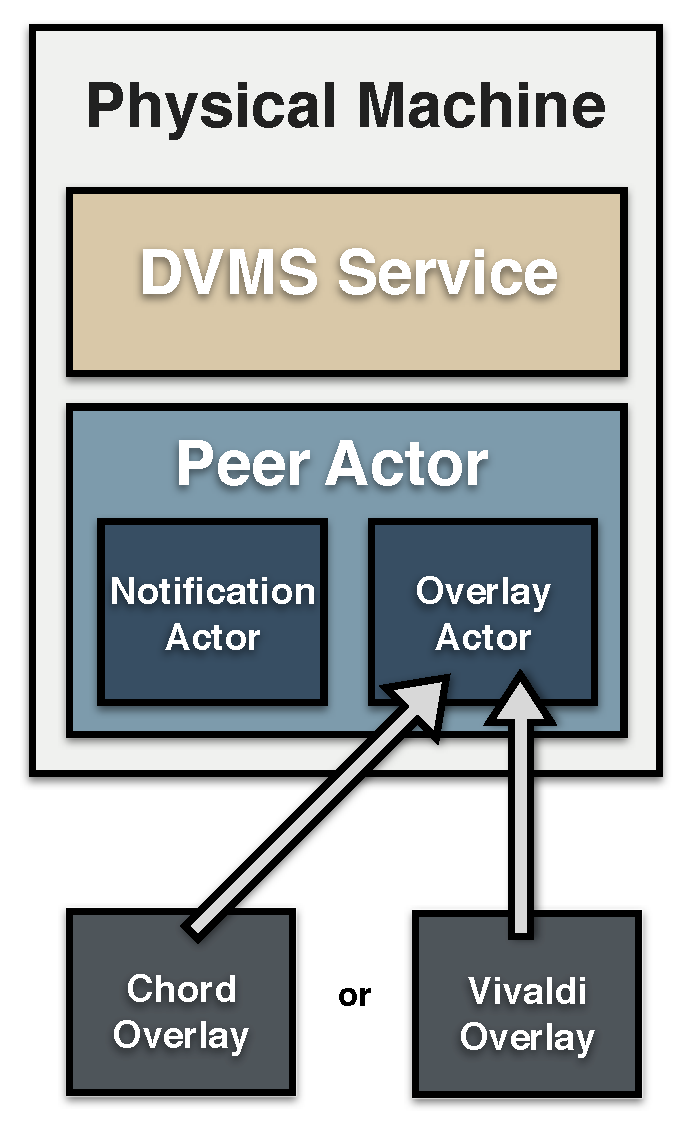
\includegraphics[width=0.5\linewidth]{Figures/DVMS.pdf}
  \caption{Architecture of DVMS based on peer actor.}%
  \label{fig:isp}%
\end{figure}




%%%% TODO: Adrien, this subsection has been already addressed in the previous subsection, so I commented it
%\subsection{Implementation of DVMS}
%
%A prototype of DVMS leveraging the \emph{peer actor} abstraction has been 
%developed. In addition we built two versions of the network overlay actor: one 
%working with Chord, and one working with the Vivaldi based overlay. This mean 
%that now DVMS is network overlay agnostic to, and thus can be used with either
%of the network overlay without requiring any modification in it's source code.
%
%The implementation is based on modern programming language and framework such as 
%\emph{Scala} and \emph{Akka framework}. Scala is a language that mixes object
%oriented programming with functional programming, it's compiler produces 
%\emph{Java bytecode} which can be run in any JVM environment. Combining Scala 
%with Akka enabled us to take advantage of advanced techniques for concurrent 
%programming such as \emph{future/promise} and \emph{actor model}, and to benefit
%from Java ease of deployment.
%


%\subsection{Grid'5000 experiments}

%\JP{Complete this section with more experimentation results.}

%\subsubsection{Objectives}
%The prototype has been tested with a various number of experiments conducted on
%the Grid'5000 testbed. 
The main objective of the experiments we conducted was to estimate the impact of locality on
the performance of a distributed scheduling algorithm. A significant portion of the
reconfiguration time is spent in live migration of virtual machines, which depends of
network parameters such as latency and bandwidth. One way to improve performance of
distributed scheduling algorithms is to promote collaboration between close ressources,
which can be reached by maximising the ratio $nb\ intrasite\ migrations/nb\ migrations$.
%\[
%	\frac{number\ of\ intrasite\ migrations}{number\ of\ migrations}
%\]


\subsection{Experimental Protocol}

To compare our experiments, we implemented a dedicated injector that makes load changes of
VMs during a predefined time. VMs are launched on PMs in a round-robin manner, \ie each
PM hosts roughly the same number of VMs at the beginning. The experiment consists in
repeatedly changes target CPU loads of VMs. Every $t$ seconds, the injector that is
deployed on a dedicated node selects one VM and changes its CPU load according to a
Gaussian distribution. $t$ is a random variable that follows an exponential distribution
with rate parameter $\lambda$. The Gaussian distribution is defined by a mean ($\mu$) as
well as a standard deviation ($\sigma$) that are given at the beginning of the experiment.
%exponential and the Gaussian distributions previously described. 
The parameters are $\lambda=\mathit{Nb\_VMs}/300$ and $\mu=70$, $\sigma=30$.
Concretely, the load of each VM starts from 0\% and varies on average every 5
min in steps of 10 (with a significant part between 40\% and 100\% of CPU
usage). Each experiment duration was set to 3600 seconds.

For each experiment, we booked 40 compute servers spread over 4 geographical sites (10
servers per site) and 1 service server from the Grid'5000 testbed. The compute servers
were used to run virtual machines and DVMS while the service node runs the aforementioned
injector.
%
Each compute node was equipped with 8 cores and hosted a number of virtual machines
proportional to its number of CPU cores ($nb VM\ =\ 1.3\ \times\ nb\ cores)$, leading to
a global number of 416 VMs. Although such a number is rather small regarding the latest
experiments that have been performed on DVMS~\cite{quesnel:ispa2013}, our goal is not to
validate once again the scalability criteria but to focus on the locality aspect of such
an algorithm.
%\[
%	number\ of\ virtual\ machines\ =\ 1.3\ \times\ number\ of\ cores
%\]

\subsection{Results}

\subsubsection{Maximization of Intra-Site Migrations}

Table~\ref{migration_table} compares the ratio between intra-site migrations and the total
number of migrations, using Chord or our locality-based overlay (LBO). The results show that the impact of locality
is significant: using LBO leads to an average number of 86.3\%
of intra-site migrations while using a Chord based DVMS decreases this ratio to 49.6\%.

\begin{table}

  \begin{center}
    \begin{tabular}{|c|c|c|}   

      % <HEADER>
      \hline \multicolumn{1}{|p{3cm}|}{ }
       & \multicolumn{1}{|p{3cm}|}{\centering Chord }  & \multicolumn{1}{|p{3cm}|}{ \centering LBO}  \\
      % </HEADER>

      % <ROW 1> => Average
      \hline
      average & 0.496 & 0.863 \\
      % </ROW 1>

      % <ROW 2> => Min
      \hline
      minimum & 0.378 & 0.798 \\
      % </ROW 2>

      % <ROW 2> => Max
      \hline
      maximum & 0.629 & 0.935 \\
      % </ROW 2>

      \hline
    \end{tabular}
  \end{center}
  \caption{\label{migration_table} Comparison of intra-site migrations ratio
    between Chord and our locality-based overlay.}
  \vspace{-0.3cm}
\end{table}


\subsubsection{Dynamic Clustering}

During our investigation of the results brought about LBO, we noticed that many of the
inter-site migrations were performed between Luxembourg and Nancy sites.
In Table~\ref{latency_table}, it is noticeable that Luxembourg and Nancy have a latency that is significantly
below usal inter-site latencies (Nancy and Luxembourg are separated by only 100 kilometers),
while Rennes and Grenoble have almost the same latency with all their respective remote sites.
Indeed, servers located in Luxembourg and Nancy are more likely to collaborate with each other, while those located
on Rennes and Grenoble will find colloborators regardless their location. This explains
why many of the inter-site migrations were performed between Luxembourg and Nancy.
This means that LBO enabled DVMS to learn which site is more interesting to perform VM
migration. Promoting low latency inter-site collaboration made many inter-site
migrations acceptable compared to those executed by the Chord version.


\begin{table}[t!]

  \begin{center}
    \begin{tabular}{|c|c|c|c|c|}   

      % <HEADER>
      \hline \multicolumn{1}{|p{2cm}|}{ } & \multicolumn{1}{|p{2cm}|}{\centering Grenoble }  & \multicolumn{1}{|p{2cm}|}{\centering Luxembourg } & \multicolumn{1}{|p{2cm}|}{\centering Nancy }& \multicolumn{1}{|p{2cm}|}{\centering Rennes } \\
      % </HEADER>

      % <ROW 1> => Grenoble
      \hline
      Grenoble & 0.09 ms & 16.55 ms & 14.24 ms & 15.92 ms \\
      % </ROW 1>

      % <ROW 2> => Luxembourg
      \hline
      Luxembourg &  & 0.17 ms & 2.70 ms & 13.82 ms \\
      % </ROW 2>

      % <ROW 3> => Nancy
      \hline
      Nancy & &  & 0.27 ms & 11.42 ms \\
      % </ROW 3>

      % <ROW 4> => Rennes
      \hline
      Rennes &  &  &  & 0.23 ms \\
      % </ROW 3>

      \hline
    \end{tabular}
  \end{center}
  \caption{\label{latency_table} Latency measured between sites.}
\end{table}


% \vspace{-1.0cm}


% \vspace{-1.3cm}

\subsubsection{Reactivity}
\begin{table}[t!]

  \begin{center}
    \begin{tabular}{|c|c|c|}   

      % <HEADER>
      \hline \multicolumn{1}{|p{3cm}|}{ }
       & \multicolumn{1}{|p{3cm}|}{\centering Chord }  & \multicolumn{1}{|p{3cm}|}{ \centering LBO}  \\
      % </HEADER>

      % <ROW 1> => Size
      \hline
      average size (servers) & 3.918 & 2.337 \\
      % </ROW 1>

      % <ROW 2> => Number of sites
      \hline
      average number of sites involved & 1.645 & 1.082 \\
      % </ROW 2>

      % <ROW 2> => Duration
      \hline
      average duration (msec) & 154.63 & 98.50 \\
      % </ROW 2>

      \hline
    \end{tabular}
  \end{center}
  \caption{\label{partitions_table} Comparison of partitions metrics between
    Chord and our locality-based overlay.}
  \vspace{-0.3cm}
\end{table}

% \vspace{-1.0cm}

Table~\ref{partitions_table} depicts metrics that allow for an objective comparison of the
efficiency of both overlay networks. Firstly, using the LBO decreases the
number of servers that are involved in partitions by 41\%, meaning that collaboration
between close nodes has become more efficient.

Secondly, it is interesting that using the LBO leads to a 
partitions duration 46\% lower than that encountered with Chord. This result is consistent with 
the fact that with our locality-aware overlay, the number of sites that are involved in partitions
becomes very close to one: collaborating with closer nodes allows
to perform scheduling/reconfiguring phases much faster since migration operations are
shorter in time, thus increasing considerably the reactivity of the system.
%% TODO (ici ca aurait ete bien de donner un odre de grandeur sur la difference entre le temps de migration intra-site vs inter-sites pour deux VMS de meme classe (i.e. qui ont la meme memory intensity, celle défini dans le code de l'injector). 

% 


\section{Related work}

\subsection{Efficient Virtual Machine Management}

Many virtual infrastructure managers have been proposed to deal with specific
concerns.
%
In this section, we will focus on some of their limitations, especially
regarding locality, scalability and fault-tolerance.

The most common managers are the centralized ones, like
Entropy~\cite{hermenier:cp11}, since they are easy to deploy.
%
They are generally designed to work on a cluster.
%
In this context, they do not take account of the network topology, and they
cannot manage VMs efficiently in a multi-site deployment.
%
Moreover, they are prone to fault-tolerance, scalability and reactivity
issues; to avoid these limitations, one possibility is to rely on more
decentralized approaches, like hierarchical or distributed ones.

Hierarchical managers, like Snooze~\cite{feller:ccgrid12}, may be more suited to
handle locality.
%
For instance, it is possible to setup (i)~one manager per cluster, and (ii)~one
(fault-tolerant) super manager that monitors cluster managers and chooses on
which cluster a new VM should start.
%
%A VM will generally stay on the cluster where it was deployed during its whole
%life cycle.
%
The main problem with this approach is that, in the absence of cooperation
between cluster managers, VMs cannot be migrated from one cluster to another,
which is especially annoying if one cluster is overloaded.
%
Moreover, the super manager is not necessarily aware of the network topology and
therefore may not be able to interact efficiently with cluster managers if the
latter are distributed among several sites.
%
Furthermore, the super manager limits the scalability of this approach; to deal
with this issue, researchers have designed distributed approaches.

Many distributed approaches have been proposed to manage
VMs~\cite{barbagallo:lncs10,feller:cloudcom12,marzolla:wowmom11,mastroianni:europar11,rouzaudcornabas:vhpc10,yazir:cloud10}.
%
Some of them are limited in terms of scalability since they (i)~require a global
view of the infrastructure to take a
decision~\cite{rouzaudcornabas:vhpc10,yazir:cloud10} and/or (ii)~rely on a
centralized service node that is not
fault-tolerant~\cite{mastroianni:europar11,yazir:cloud10}.
%
Some approaches lead to a huge number of
migrations~\cite{barbagallo:lncs10,mastroianni:europar11} without necessarily
optimizing the chosen scheduling criterion~\cite{barbagallo:lncs10}.
%
Moreover, none of these approaches have been designed to take account of the
network topology and therefore manage VMs efficiently in a multi-site
deployment.

To summarize, a locality-aware distributed approach is required to (i)~avoid
issues related to scalability and single points of failures, and to (ii)~manage
VMs efficiently in heterogeneous network environments like those found in
multi-site deployments.

\subsection{P2P}




Cloud Computing has entered our everyday life at a very high speed and huge scale. From classic high performance computing simulations to the management of huge amounts of data coming from mobile devices and sensors, its impact can no longer be minimized. While a lot of progress has already been made in Cloud technologies, there are several concerns that limit the complete adoption of the Cloud Computing paradigm.

In a previous report~\cite{lebre:hal-00854204}, we outlined that, in addition to these concerns, the current model of UC is limited by intrinsic issues. Instead of following the current trend by trying to cope with existing platforms and network interfaces, we proposed to take a different direction by promoting the design of a system that will be efficient and sustainable at the same time, putting knowledge and intelligence directly into the network backbone itself. The innovative approach we introduced will definitely tackle and go beyond Cloud Computing limitations. Our objective is to pave the way for a new generation of Utility Computing that better matches the Internet structure by means of advanced operating mechanisms. By offering the possibility to tightly couple UC servers and network backbones throughout distinct sites and operate them remotely, the LUC OS technology may lead to major changes in the design of UC infrastructures as well as in their environmental impact. The internal mechanisms of the LUC OS should be topology dependent and resources efficient. The natural distribution of the nodes through the different points of presence should be an advantage, which allows to process a request according to its scale: Local requests should be computed locally, while large computations should benefit from a large number of nodes.

The first step toward this highly distributed Cloud infrastructure taking into account locality and network distance is the scheduling of VMs taking into account locality. Thus is this paper, we presented our first building block of our distributed Cloud infrastructure that consists in using P2P algorithms and a vivaldi overlay connected to DVMS, an efficient and flexible VMs scheduler. Our first experiments over Grid'5000 show that, connecting 4 differents sites and scheduling VMs over them, we can gain up to 66\% of inter-sites operations. 

Our future work will consist in ... 

%\input{intro}
%\input{related}
%\input{approach}
%%%%
\section{Premises of a LUC OS: The \discovery Proposal\label{sec:archi}}

In this section, we propose to go one step further by discussing preliminary
investigations around the design and the implementation of a first LUC OS
proposal: the \discovery system (DIStributed and COoperative Management of
Virtual EnviRonments autonomouslY). We draw the premises of the \discovery
system by emphasizing some of the challenges as well as some research directions
to solve them. Finally, we give some details regarding the prototype that is
under development and how we are going to evaluate it.  

\subsection{Overview}

The \discovery system relies on a multi-agent peer-to-peer system deployed on
each physical resource composing the LUC infrastructure. Agents are autonomous
entities that collaborate to efficiently use the LUC resources. In our context,
efficiency means that a good trade-off is found between satisfying user's
expectations, ensuring reliability, reactiveness as well as availability of the
services while limiting the energy consumption of the system and providing
scalability. We propose thus to leverage P2P techniques, that
allow self-* properties, such as self-adaptation and self-repairing of overlays. 
%
To reduce the management complexity as well as the design and the
implementation of the different mechanisms that are mandatory, we strongly
support to use micro-kernel concepts. Such an approach should enable to design
and implement services at higher level while leveraging P2P mechanisms
at the lower ones.  Furthermore, to address the different objectives and reduce
the management complexity, we also underline that self-* properties should be
present at every level of the system.  We think that relying on a multi-agent
peer-to-peer system is the best solution to cope with the scale as well as the
network disconnections that may create temporary partitions in a LUC platform.

In \discovery, each agent has two purposes: (i) maintaining knowledge base on the
LUC platform composition (ii) ensuring the correct execution of the VEs. 
Concretely, the knowledge base will consist of overlays that will be used 
for the autonomous management of the
VEs life cycle. This includes the configuration, deployment and monitoring of
VEs as well as the dynamic allocation or relocation of VMs to adapt to changes
in VEs requirements and physical resources availability. To this end, agents
will need to rely on dedicated mechanisms that can be classified as follows: 

\begin{itemize}
\item Mechanisms related to physical resource localization and monitoring, 
\item Mechanisms related to VEs management, 
\item Mechanisms related to the VM images management, 
\item Mechanisms related to reliability,
\item Mechanisms related to security and privacy.
\end{itemize}

\subsection{Resource Localization and Monitoring Mechanisms\label{ssec:p2p}}

Keeping in mind that \discovery should be designed in a fully distributed way,
most of the mechanisms should build on top of overlays in order to abstract changes
that occur at the physical levels. The specific requirements of this platform
will lead to develop a particular kind of overlays, having minimalism in mind.

More concretely, the first step is to design, at the lowest level, a first
overlay layer intended to abstract out the details of the physical routes and
computing utilities, while satisfying the basic topology requirements needed --
locality and availability. This overlay needs to enable the communications
between any two nodes in the platform. While overlay computing has been
extensively studied over the last decade, we emphasize here on minimalism, and
one particular feature with regard to the envisioned platform described before:
retrieving physically close nodes from a given starting node.

\subsubsection*{Giving nodes a position}

The physical network's connections are considered as arbitrary. We choose to
rely on the Vivaldi protocol~\cite{dabek:2001:sigcomm04}. Vivaldi is a
distributed algorithms assigning coordinates in the plane to nodes of a
distributed systems, each node being equipped with a \emph{view} of the network,
\emph{i.e.}, a set of nodes it knows. This view is initially assumed as
arbitrary. Coordinates obtained by a node reflects its \emph{position} in the
network, \emph{i.e.}, close nodes in the network are given close coordinates in
the plane. This is achieved by every node periodically checking the round trip
time between itself and another node (from its view, a different one at each
step) and adapting its distance (by changing its coordinates) with this node in
the plane accordingly. 

\begin{figure}
  \begin{minipage}[c]{.45\linewidth}
	\vspace*{.5cm}
   \hspace*{-0.5cm}
      	\centering 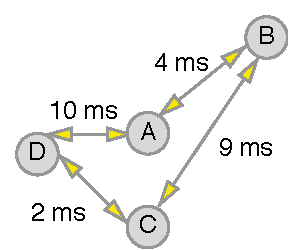
\includegraphics[width=4cm]{./FIGS/vivaldi_before.pdf}

   \hspace*{0.5cm}
	\vspace*{.4cm}
		\caption{Vivaldi plot before updating positions.}
		{\small Each node ping other nodes. Each node maintains a map of distance.}
\label{fig:vivaldi_before}
   \end{minipage}
\hspace*{0.6cm}
   \begin{minipage}[c]{.45\linewidth}
   	\centering 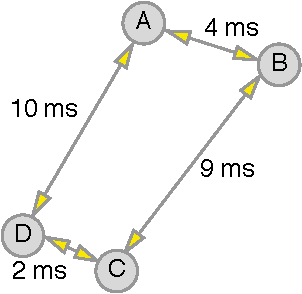
\includegraphics[width=4cm]{./FIGS/vivaldi_after.pdf}
	\vspace*{0.20cm}
		\caption{Vivaldi plot after updating positions.}
		\label{fig:vivaldi_after} 
{\small The computed positions of other nodes are periodically updated.}
  \end{minipage} \hfill
\end{figure}

\newpage

Note that a global accurate positioning of nodes can be
obtained if nodes have a few long-distance nodes in their
view~\cite{dabek:2001:sigcomm04}. These long distance links can be easily
maintained through a simple gossip protocol.

\subsubsection*{Searching for close nodes}

Once this map is achieved (each node its coordinates), we are able to decide
whether two nodes are close by calculating their distance. However, the view of
each node does not \emph{a priori} contain its closest nodes. We need additional
mechanisms to locate a set of nodes that are close to a given initial node --
Vivaldi gives a \emph{location} to a node, but not a neighborhood. To achieve
this, we use a modified distributed version of the classic Dijkstra's algorithms
used to find the shortest path between two nodes in a graph. The goal is to
build a \emph{spiral}\footnote{The term \emph{spiral} is here a misuse of
language, as there is no guarantee that the graph actually drawn in the plane
does not contain crossing edges. The only guarantee is that when following the
path constructed, the nodes are always further from the initial node.}
interconnecting the nodes in the plane that are closest to a given initial
node. Let us consider our starting point is node $s$. The first step is to find
a node to build a two-node spiral with $s$. Such a node is sought in the current
view of $s$ by selecting the node, say $a$, having the smallest distance with
$s$. By contacting $a$, $s$ then sends its view to $a$, $s$ stores $a$ as its
successor in the spiral, and $a$ adds $s$ as its predecessor in the spiral. Then
$s$ forwards its view to $a$. $a$ then creates a new view by keeping the $n$
node which are closest to $a$ in both $s$ and $a$'s views. This last view is
then referred to as the \emph{spiral view} and is intended to contain a set of
nodes in which to find the next step of the spiral. Then $a$ restarts the same
process: Among the spiral view, it chooses the node with the smallest distance
to $s$, say $b$, and adds it in the spiral -- $a$ becomes the predecessor of $b$
and $b$ becomes the successor of $a$. Then, the spiral view is sent to $b$ which
updates it with the nodes it has in its own view. The process is repeated until
we consider we have gathered enough nodes with regard to the requesting
application.

One risk to be mitigated is not to blocked by a spiral view containing only
nodes that are already in the spiral. However, this problem can be easily
addressed by forcing the presence of a few long distance nodes whenever it is
updated.

\subsubsection*{Learning}

Applying the protocol described above, the quality of the spirale is
questionable in the sense that the nodes that are actually close to the starting
point node $s$ may not be included. The only property ensured is that one step
forward the path built always takes us further from the starting point node.

To improve the \emph{quality} of the spiral, \emph{i.e.}, reduce the average
distance between the nodes it comprises and the initial node, we add a learning
mechanism coming with no extra communication cost, as it does not require any
extra message. When a node is contacted for becoming the next node in one
spiral, and receives the associated spiral view, it can also keep the nodes that
are closest to itself, thus potentially increasing the quality of a future
spiral construction.

\subsubsection*{Routing}

Still based on the minimal design, and independently from the spiral
constructions, there is a need for routing.

\ftodo[CT]{TODO}

% Each node doing so in parallel, a number of clusters are created inside which we
% can ensure a certain level of locality -- all nodes inside this group can
% communicate with each other very efficiently. Given the number of nodes in these
% groups, the inner topology of a group can either rely on very simple graphs,
% such as rings, or more connected graphs, to accelerate the dissemination and
% retrieval of information in the group. Note that, still based on simple
% gossiping techniques, such graphs can be easily maintained as the network's
% conditions change. For instance, if a link becomes overloaded, the other nodes
% will react to this change by removing nodes with which they communicate through
% this link from their local group. Such groups are exemplified on
% Figure~\ref{fig:renater_overlay} (for the west part of the platform).

% \begin{figure}[htbp]
% 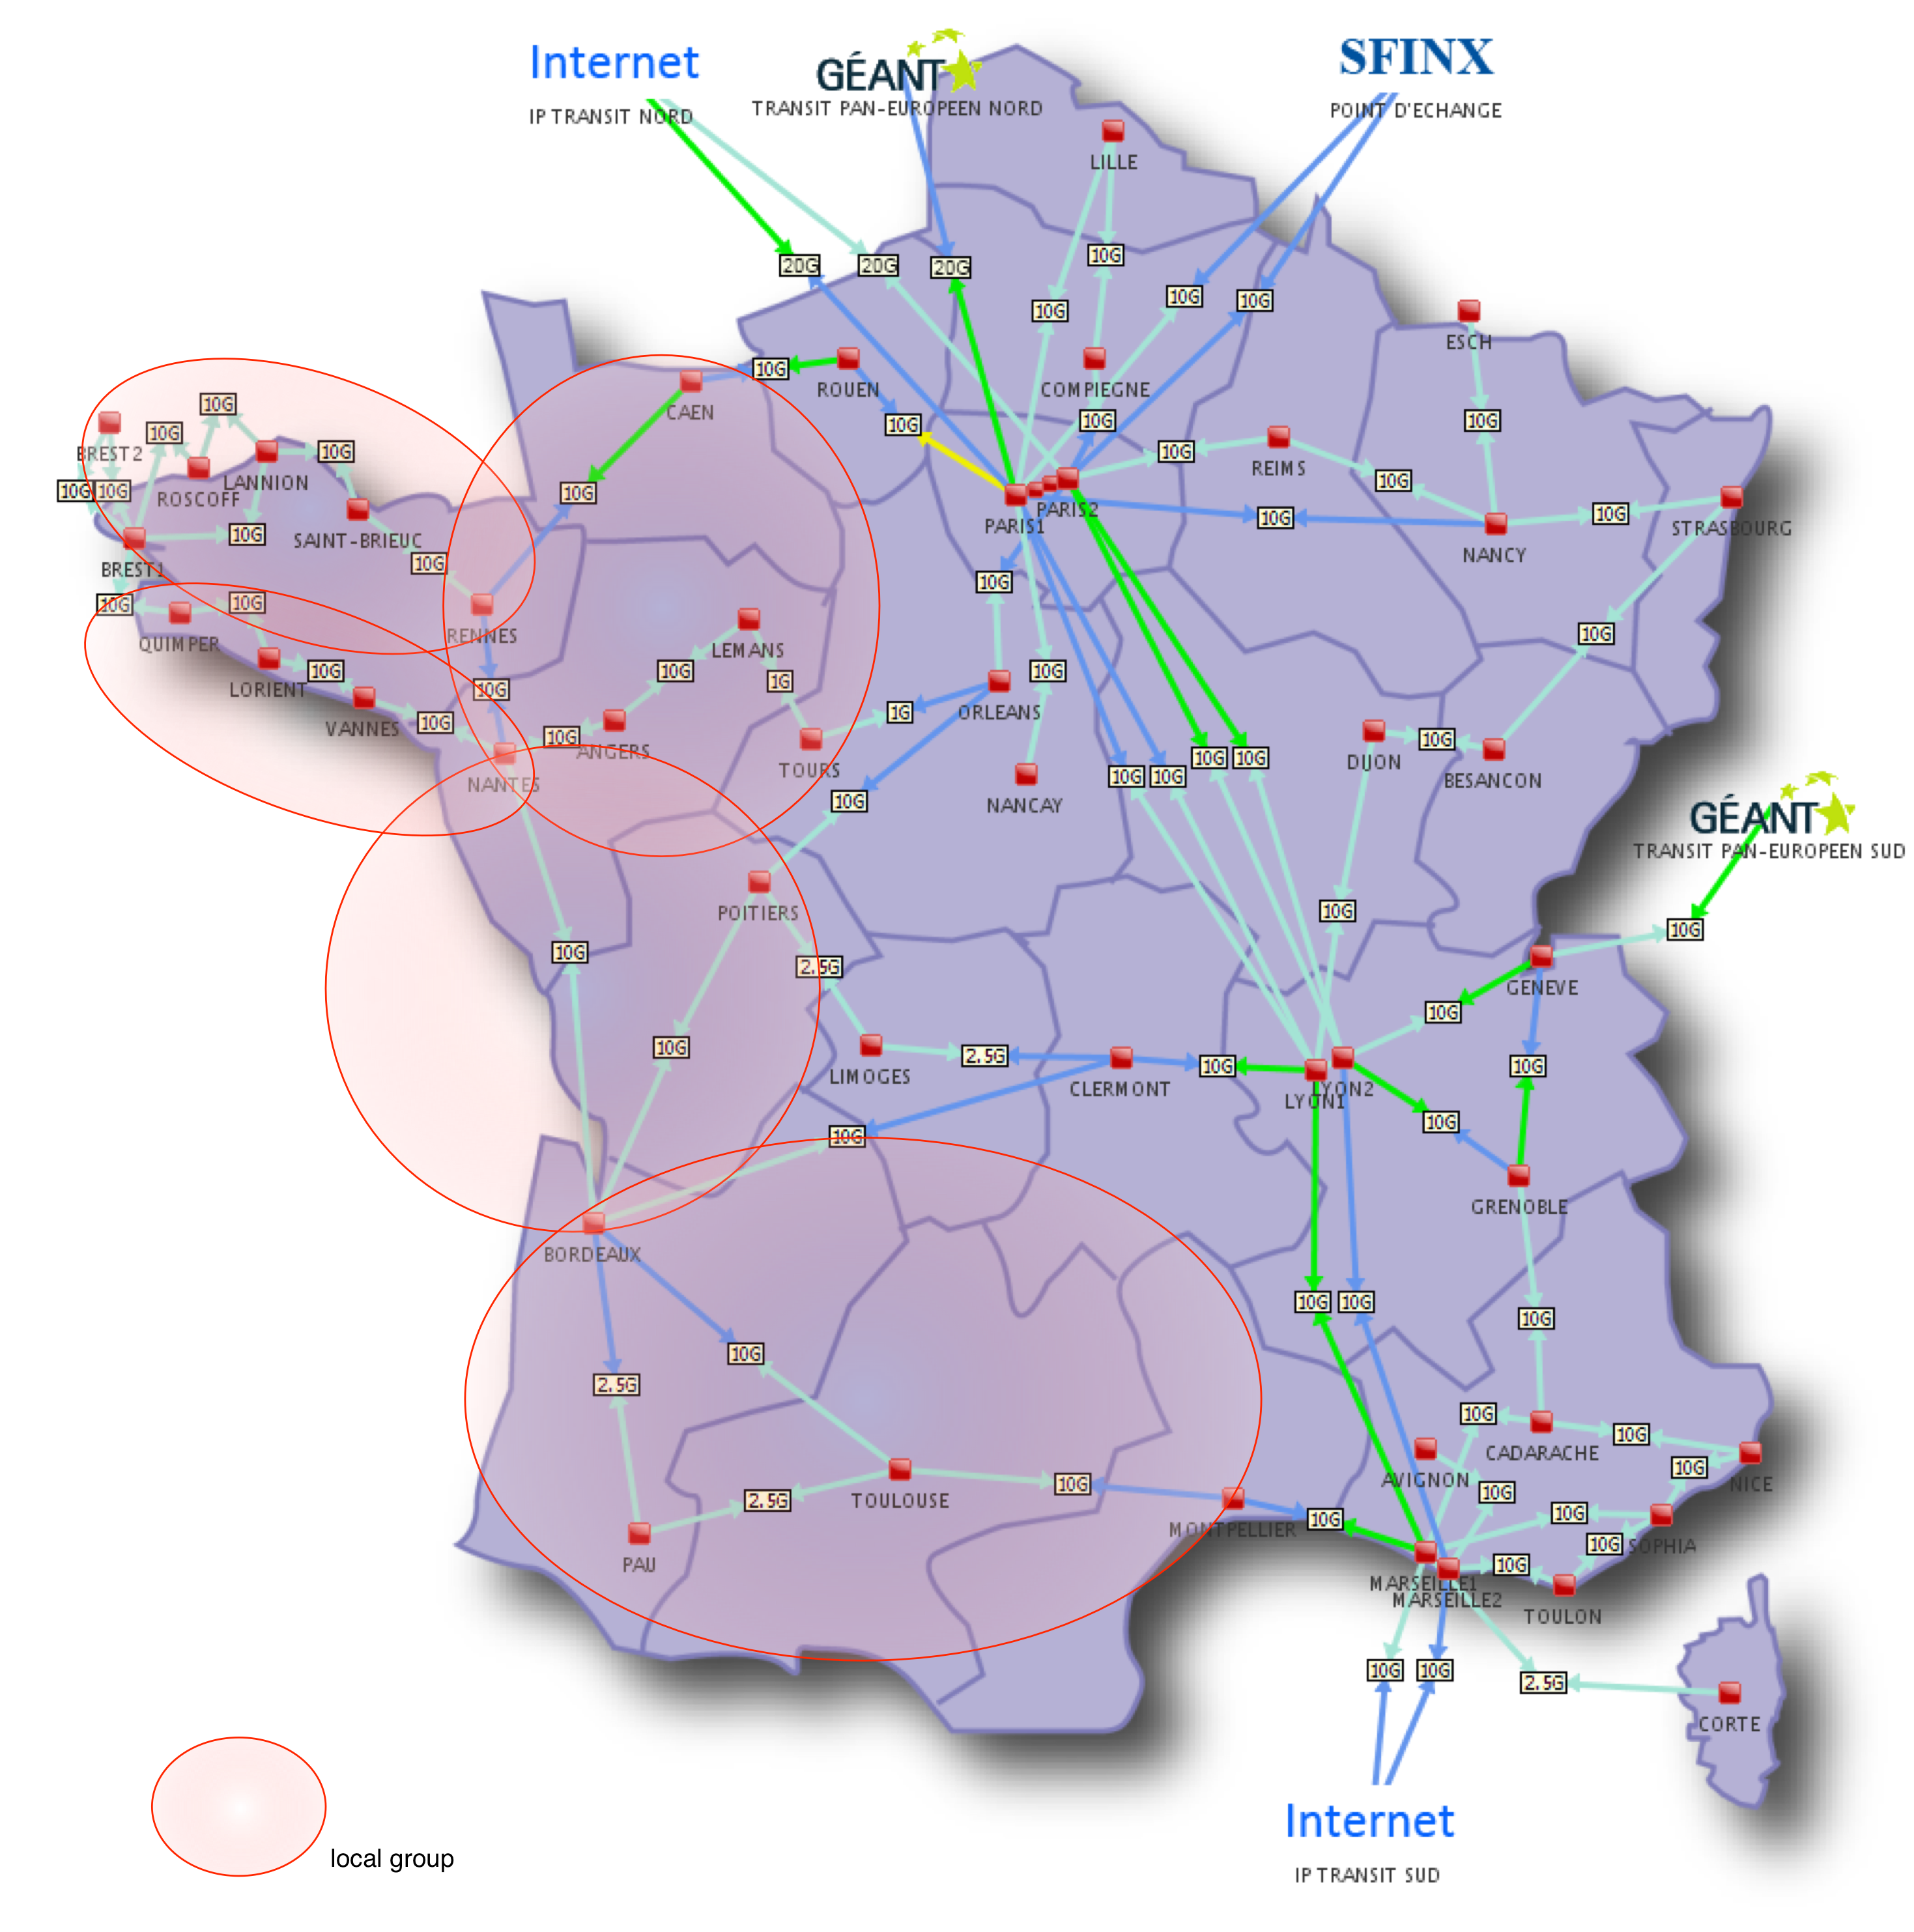
\includegraphics[width=12cm]{./FIGS/renater_overlay.png}
% \caption{Overlay local groups on top of the RENATER platform.\label{fig:renater_overlay}}
% \end{figure}

% As we can see on Figure~\ref{fig:renater_overlay}, it follows from the way the
% overlay is built that some nodes may be a member of several groups. The Nantes
% site for instance is part of three of these groups, given its
% physical position. More generally, the overlay will take the shape of a set of
% groups with some \emph{bridges} between the groups. Note that several
% \emph{bridges} can interconnect two local groups. Thus, any request first goes
% through local nodes allowing for its local processing, and avoiding the need for
% global coordination mechanisms.

% To be able to localize a particular VM, the system has to be able to route a
% request from any node to any other node. This functionality is the classic
% problem of P2P overlays, which is traditionally solved in structured overlay networks by
% maintaining a routing table on each node, and by a flooding mechanism or with
% random walks in unstructured overlays. These techniques are usually designed for
% very large scale networks with different guarantees and costs. Here, given the
% particular ``intermediate'' scale of the platform, and its specific
% requirements, we believe that these existing techniques are too
% \emph{powerful}. As we want to design a minimalistic overlay, there is room to
% try to design a new routing technique specifically fitting our
% requirements. The aim is then to maintain, in all groups, information about the
% distance between this group and \emph{close} groups in terms of number of bridge nodes
% to go through. Hence, the system will be able to route quickly between \emph{close}
% groups. The routing of requests between \emph{far} groups will be based on a random
% decision when no information are available, but \emph{oriented} by the aim of
% going away from the request's source.

% This overlay will provide the basic building block of the platform, on which will
% rely higher level overlays and functionalities, which are described in the
% following sections.

% \subsubsection*{Upper-Layer overlays}

% \ftodo[CT]{To be completed...}


% \ftodo[AL]{To be completed by Cedric and Marin}
% \ftodo[AL]{C/P from the proposal : 
% self-organizing overlay construction mechanisms based on gossip and epidemic
% techniques that will link the \discovery resources in navigable graphs onto
% which requests for VE can be routed and allocated. It will investigate
% mechanisms to quickly adapt these graphs to changing conditions and
% infrastructure, and mechanisms to monitor the adequacy of previous requests
% solutions to these changing conditions as these occur.}

\subsection{VEs Management Mechanisms}
\label{ssec:vem}
In the \discovery system, we define a VE as a set of VMs that may have specific
requirements in terms of hardware, software and also in terms of placement:~
some VMs must be on the same node/site in order to cope with performance objectives while
others should not be collocated in oder to ensure
high-availability criteria~\cite{hermenier:2013}.
As operations on a VE may occur in any place from any location, each agent should provide the capability
to configure and start a VE, to suspend/resume/stop it, to relocate some of its VM if need be or simply to retrieve the location of a particular VE. 
Most of these mechanisms are integrated on current UC platforms. However as mentioned, they
should be revisited to correctly run on the infrastructure we target
(\textit{i.e.} in terms of scalability, resiliency and reliability).
To this aim, the \discovery system relies on the aforementioned P2P mechanisms. 
As a first example, placing the VMs of a VE requires to be able to find available nodes that
fulfills the VM needs (in terms of resource needs as well as placement
constraints). Such a placement can start locally, close to the client
application requesting it, \textit{i.e.}, in its local group. If no such node is
found, simple navigation ensures that the request will encounter a bridge
eventually, leading to the exploration of further nodes. This navigation goes
on until one sufficiently available node is found.
A similar process is performed by the mechanism in charge of  dynamically
controlling and adapting the placement of VEs during their lifetime.  For instance, in
order to ensure particular needs of a VM, it can be necessary to relocate other
ones. According to the predefined constraints of VEs, some VMs might be
relocated on far nodes while other would prefer to be suspended.  Such a
mechanism has been deeply studied and validated in the DVMS
mechanism~\cite{dvms:wiki,quesnel:2012}. DVMS (Distributed Virtual
Machines Scheduler) enables to dynamically schedule a significant number of VMs
throughout a large-scale distributed infrastructure while guaranteeing VM
resource expectations.  

A second example regards the configuration of the network elements of a VE. 
Although it might look simple, assigning the right IPs to
each VM as well as maintaining the intra-connectivity of a VE becomes a bit more complex than in
the case of a single network domain, \textit{i.e.} a mono-site deployment.
%
Keeping in mind that a LUC infrastructure is
by definition spread WANwide, a VE can be hosted between distinct network
domains during its lifetime. No solution has been chosen yet. 
Our first investigations led us to leverage techniques
such as the IP over P2P project \cite{ganguly:2006}. However, the definition of
software network becomes more and more important. Investigating proposals such as
the Open vSwitch project \cite{pfaff:2009} looks a promising direction to solve such issue.
%

\subsection{VM Images Management}

In a LUC infrastructure, VM images could be deployed in any place from any
other location, but being in a large-scale, heterogeneous and widely spread
environment makes the management of VM images more difficult than more
conventional  centralized repositories.  
At coarse grain, the management of the VM images should be (i) consistent
with regards to the location of each VM throughout the \discovery infrastructure and
(ii) reachable in case of failures.
%
The envisioned mechanisms dedicated to the management of the VM images have been
classified into two sub-classes.
%
First, it will be mandatory to deliver appropriate mechanisms to efficiently
upload and replicate VM images among a high number of nodes in order to ensure
efficiency as well as reliability.  Second, the \discovery system should 
include specific mechanisms devoted to the scheduling of the VM image
transfers. Advanced policies are important to improve the efficiency of each
transfer that may occur either at the boot time or during VM relocations. 

Regarding storage and replication mechanisms,  an analysis of an IBM Cloud concludes
that a fully distributed model using P2P technology is not the best choice to manage VM images as the
number of instances of the same VM image is rather small~\cite{peng:2012}. However, central or
hierarchical solutions are not suited for the infrastructure we target.
Consequently, an augmented P2P solution working with replicas and
deduplication will have to be investigated in order to provide more
reliability, speed, and scalability to the system. For example, analyzing
different VM images shows that at least 30\% of the image is shared between
different VMs. This 30\% can become a 30\% space reduction, a
30\% increased reliability or a 30\% of speed increase. Depending on the
situation, we should decide to go from one scenario to another. 
%Finally, the number of replicas and deduplicated data should be dynamically balanced.

Regarding the scheduling mechanisms, it has been shown that a storage system with VMs being used by I/O intensive tasks 
can increase boot time from 10 to 240 seconds \cite{tan:2008}. Some actions like providing the
image chunks needed to boot first~\cite{tang:2011}, defining a new
image format, and pausing the rest of the I/O operations, can provide a
performance boost and limit the overhead that is still observed in commercial
Clouds~\cite{mao:2012}. 
%These actions should also take into account
%power-like metrics in order to reduce the energy consumption of data transfers.
%According to (Preist et Shabajee Nov 2010) the cost to transmit 1 MB can be of
%4Wh. Considering the size of VM images, any improvement aiming at reducing
%data movement will make a big difference.

More generally, the amount of data related to VM images is significant.
Actions involving data  should be aware of their implications on metrics like
(but not limited to): energy efficiency, bandwidth, reliability, proximity, and
hardware usage. The scheduler could also anticipate actions like moving images when
the load is low or the energy is cheaper.

%% \subsection{Reliability Mechanisms}
%% %These mechanisms should ensure  reliability and high availability of the
%% %\discovery system despite the scale and dynamicity of the underlying physical
%% %infrastructure.   
%% By nature, a LUC is a highly distributed platform where 
%% node and network failures will be much more frequent than in
%% actual UC platforms.  Furthermore, since resources could be located anywhere,
%% the expected mean time to repair failed equipments might be much larger than in
%% other platforms. For all these reasons, a set of dedicated mechanisms should be designed in order
%% to provide a fully transparent failure management with minimum downtime. 
%% %
%% To this aim, the \discovery system should include, first,  mechanisms in charge of its own reliability. 
%% Such mechanisms are required to avoid losing or corrupting important information
%% regarding the state of the system.  Of course, handling all kinds of failures
%% and implementing a fully resilient operating system is a complex task. Hence,
%% we propose to consider in a first time a crash-stop failure model. In other words, the
%% \discovery system should be able to autonomously restart any service by
%% relocating it on an healthy agent each time it is mandatory.  This implies to
%% define a common design pattern, \textit{i.e.} a set of recommendations, that each
%% service should follow to ensure such characteristics. Besides, in order to
%% ensure that such a pattern may be applied to stateful services, the system can
%% require a Cassandra like system \cite{lakshman:2010} that provides reliable and highly available
%% storage for critical system states. Retrieving the information related to one
%% service need to rely on the kind of mechanisms described in Section~\ref{ssec:p2p}.

%% %
%% In addition to be robust enough, the \discovery system should ensure the
%% reliable execution of virtual environments. The first mechanisms consists in
%% using snapshotting capabilities delivering by virtualization technologies.
%% Concretely, each internal states of a VM should be periodically saved on a
%% persistent storage.  When a crash occurs on a VM, its associated VE can be
%% restarted from the latest consistent states, \textit{i.e.} all VMs of the VE will be
%% resume for their latest snapshot.  As for the other mechanisms, performing VM
%% snapshotting in a large-scale, heterogeneous and widely spread environment is a
%% challenging task. However, we believe that aforementioned mechanisms in charge
%% of the VM images as well as recent proposals \cite{nicolae:2011} might enable
%% to provide such a feature. 
%% Although VM snapshotting provides a first level of reliability, it is not
%% sufficient to ensure high availability of the VE. More advanced mechanisms must
%% be proposed.  Our idea is to include mechanisms based on primary-backup
%% replication techniques. 
%% The basic principle is to have one active replica of the VM (the primary)
%% sending state updates to the other replicas (the backups) periodically. If the
%% primary fails, one of the backup can resume the execution transparently for the
%% outside world. Furthermore since the entire VM is replicated, applications can
%% be run unmodified.  Solutions to replicate VMs inside a cluster have been
%% proposed. However efficiently replicating VMs over a WAN is a huge challenge.
%% Limiting the size of the backup updates\cite{rajagopalan:2012}, and
%% reducing the impact of the required synchronizations on the execution of the
%% primary \cite{gerofi:2012}  are research directions to be further
%% studied. A better understanding of the parts of a VM that really need to be
%% updated is required. It might require to trade transparency for performance by
%% allowing latency-sensitive applications to define which part of their state has
%% to be updated.

%% \ftodo[AL]{Integrate the P2P aspect into the reliability section}
%% \subsubsection*{Monitoring Example}

%% Another key use of this low-level overlay is proactive replication of VMs,
%% keeping in mind that two identical VMs should be placed in relatively distant
%% nodes, for fault-tolerance reasons (close nodes have a high probability to fail
%% together). Following the defined overlay structure, this can be done through a
%% navigating scheme where at least one bridge is encountered. Monitoring this
%% replica can be done easily by having a \emph{watcher} in the same local group as
%% the replica.

\subsection{Reliability Mechanisms}
%These mechanisms should ensure  reliability and high availability of the
%\discovery system despite the scale and dynamicity of the underlying physical
%infrastructure.   
In a LUC, failures will be much more frequent than in actual UC
platforms. Furthermore, since resources could be highly distributed,
the expected mean time to repair failed equipments might be much
larger than in other UC platforms. For all these reasons, a set of
dedicated mechanisms should be designed in order to provide fully
transparent failure management with minimum downtime. 

%% It includes
%% mechanisms to ensure the high availability of the \discovery system
%% itself and mechanisms to allow executing VEs reliably.

Ensuring the high availability of the \discovery system requires being able to
autonomously restart any service by relocating it on a healthy agent each time
it is mandatory. To avoid losing or corrupting important information regarding
the state of the system, a Cassandra-like system~\cite{lakshman:2010} is
required to provide a reliable and highly available back-end for stateful
services.

Regarding VEs reliability, a first level of fault tolerance can be
provided by leveraging VMs snapshotting capabilities. Periodical
snapshots will allow restarting the VE from its last snapshot in the
event of a failure. Performing VM snapshotting in a large-scale,
heterogeneous, and widely spread environment is a challenging
task. However, we believe that adapting recently proposed
ideas~\cite{nicolae:2011} in this field would allow us to provide such
a feature.

Snapshotting is not enough for services that should be made highly
available, but a promising solution is to use VM
replication~\cite{Petrovic2012}. To implement VM replication in a WAN,
solutions to optimize synchronizations between
replicas~\cite{gerofi:2012,rajagopalan:2012} should be
investigated. Also, we think that a LUC has the major advantage over
other UC platforms, that it is tightly coupled with the network
infrastructure. As such, we can expect \emph{low} latencies between
nodes and so, to be able to provide strong consistency between
replicas while achieving acceptable response time for the replicated
services. 
%Note that the overlays presented in Section~\ref{ssec:p2p}
%for replicas localization and monitoring. Locating replicas based on a
%navigating scheme where at least one bridge is encountered, would be
%enough to ensure that they have a low probability to fail
%simultaneously.


Reliability techniques will of course make uses of the overlays
for resource localization and monitoring. 
Replicated VMs should be hosted on nodes that have a low
probability to fail simultaneously. Following the previously defined
overlay structure, this can be done through a navigating scheme where
at least one bridge is encountered. Monitoring a replica can then be
done by having a \emph{watcher} in the same local group as the
replica.

%% Another key use of this low-level overlay is proactive replication of VMs,
%% keeping in mind that two identical VMs should be placed in relatively distant
%% nodes, for fault-tolerance reasons (close nodes have a high probability to fail
%% together). Following the defined overlay structure, this can be done through a
%% navigating scheme where at least one bridge is encountered. Monitoring this
%% replica can be done easily by having a \emph{watcher} in the same local group as
%% the replica.




%
%% To this aim, the \discovery system should include, first,  mechanisms in charge of its own reliability. 
%% Such mechanisms are required to avoid losing or corrupting important information
%% regarding the state of the system.  Of course, handling all kinds of failures
%% and implementing a fully resilient operating system is a complex task. Hence,
%% we propose to consider in a first time a crash-stop failure model. In other words, the
%% \discovery system should be able to autonomously restart any service by
%% relocating it on an healthy agent each time it is mandatory.  This implies to
%% define a common design pattern, \textit{i.e.} a set of recommendations, that each
%% service should follow to ensure such characteristics. Besides, in order to
%% ensure that such a pattern may be applied to stateful services, the system can
%% require a Cassandra like system \cite{lakshman:2010} that provides reliable and highly available
%% storage for critical system states. Retrieving the information related to one
%% service need to rely on the kind of mechanisms described in Section~\ref{ssec:p2p}.

%% %
%% In addition to be robust enough, the \discovery system should ensure the
%% reliable execution of virtual environments. The first mechanisms consists in
%% using snapshotting capabilities delivering by virtualization technologies.
%% Concretely, each internal states of a VM should be periodically saved on a
%% persistent storage.  When a crash occurs on a VM, its associated VE can be
%% restarted from the latest consistent states, \textit{i.e.} all VMs of the VE will be
%% resume for their latest snapshot.  As for the other mechanisms, performing VM
%% snapshotting in a large-scale, heterogeneous and widely spread environment is a
%% challenging task. However, we believe that aforementioned mechanisms in charge
%% of the VM images as well as recent proposals \cite{nicolae:2011} might enable
%% to provide such a feature. 
%% Although VM snapshotting provides a first level of reliability, it is not
%% sufficient to ensure high availability of the VE. More advanced mechanisms must
%% be proposed.  Our idea is to include mechanisms based on primary-backup
%% replication techniques. 
%% The basic principle is to have one active replica of the VM (the primary)
%% sending state updates to the other replicas (the backups) periodically. If the
%% primary fails, one of the backup can resume the execution transparently for the
%% outside world. Furthermore since the entire VM is replicated, applications can
%% be run unmodified.  Solutions to replicate VMs inside a cluster have been
%% proposed. However efficiently replicating VMs over a WAN is a huge challenge.
%% Limiting the size of the backup updates\cite{rajagopalan:2012}, and
%% reducing the impact of the required synchronizations on the execution of the
%% primary \cite{gerofi:2012}  are research directions to be further
%% studied. A better understanding of the parts of a VM that really need to be
%% updated is required. It might require to trade transparency for performance by
%% allowing latency-sensitive applications to define which part of their state has
%% to be updated.

%% \ftodo[AL]{Integrate the P2P aspect into the reliability section}
%% \subsubsection*{Monitoring Example}

%% Another key use of this low-level overlay is proactive replication of VMs,
%% keeping in mind that two identical VMs should be placed in relatively distant
%% nodes, for fault-tolerance reasons (close nodes have a high probability to fail
%% together). Following the defined overlay structure, this can be done through a
%% navigating scheme where at least one bridge is encountered. Monitoring this
%% replica can be done easily by having a \emph{watcher} in the same local group as
%% the replica.


\subsection{Security and Privacy Mechanisms}
%
%LUC OS should include a mechanism for the security of the lower layers and particularly multiple P2P overlays.
%% Previous research~\cite{sybilattacks} has shown that without trusted identities, it 
%% is not possible to protect a P2P overlay against sybil attacks. 
%Recent advances~\cite{Castro:2002:SRS:844128.844156} in DHT 
%security might enable to provide a secured overlay. 
%But they are not sufficient to ensure the good behavior of resources and users.
%LUC OS should include an authentication and certification mechanism that 
%evaluates the behavior of resources and VEs.
%% Finally, as the resources could be hosted in more or less secured locations and provided by different 
%% resource providers, this certification should also be used to rank the security of each resources.
%% \ftodo[AL->JRC]{Could you please put only the most relevant one}
%
%Moreover, LUC OS shoud integrate security decision and enforcement points (SDEPs).
%%  mechanisms at all locations and layers.
%To guarantee a security, 
%Sandhu~\cite{sandhu_towards_2010} propose a roadmap towards such security mechanisms for
%Cloud where the Cloud infrastructure provides security hooks and
%mechanisms. 
%% To realize this goal, they point out the need for
%% \emph{developing models, methodologies and architectures for
%%   decentralized dynamic management of security and assurance
%%   policies}. 
%Similarly than other mechanisms, 
%As LUC infrastructure is even more distributed, heterogeneous and 
%dynamic than Cloud, its SDEPs should be distributed and 
%decentralized and able to evolve according to security requirements 
%without central security decision points. Futhermore, 
%LUC OS should provide a protocol to ease the collaboration between the SDEPs.
%Indeed, when new resources join
%a LUC infrastructure, SDEPs from different locations 
%must collaborate to extend the LUC infrastructure while keeping it secured. This collaboration between 
%SDEPs will also append when a VE is spread over different 
%resources and/or migrate from one to another.
%
%LUC OS should allow users to express their security requirements on their VEs.
%The expression of these requirements itself is a complex task.
%% LUC OS must propose to the user a way to model their VEs and 
%% the security requirements on them. 
%To ease the expression of these 
%requirements, LUC OS must propose a domain specific security language 
%that defines high-level security requirements such as \cite{rouzaud_book13b,Bacon:2010:EEA:2023718.2023739} do 
%for Clouds. These security requirements will be enforced 
%by SDEPs during the whole life time of the VE.
%
%%%%
% 1./ Securiser les overlays
% 3.a./ Definir  un DSL pour les VEs
% 3.b/ Offrir des moyens d'integrer des SDEPs (i.e. moulinette qui maintient/execute les DSLs)
% 2./ Securiser l'acces aux operations de manipulation de l'infra (admin et user)

% 1
To be successful, \discovery needs to provide mechanisms and methods to construct trust relationships between resource providers.
Trust relationships are known to be complex to build~\cite{Miller:2010:TWT:1907636.1907726}. Providing strong authentication, assurance and certification mechanisms for 
providers and users is required but it is definitely not enough. Trust covers socio-economic aspects that must be covered but are out of the scope of this chapter.
The challenge is to provide a trusted \discovery base.

% 2 
As overlays are fundamentals for all \discovery mechanisms, the first challenge is to ensure
that they are not compromise. Recent advances~\cite{Castro:2002:SRS:844128.844156} might enable to tackle such concerns.

%3.A ? 
The second challenge will consist in providing end-users with a way to define their own  security policies and to ensure that such policies are enforced. 
The expression of these requirements itself is a complex task.
The challenge is to improve the current trade-off between security and usability.
To ease the expression of these policies, we are currently defining a  domain specific security language
that defines high-level security requirements \cite{rouzaud_book13b,alefray:hpdc:2013}. 
These security policies will be enforced in a decentralize manner
by distributed security decision and enforcement points (SDEPs) during the whole lifetime of the VE.
Implementing such SDEP mechanisms in a distributed fashion will require to
conduct specific research as they are currently only prospective proposals for
classic UC infrastructures~\cite{Bacon:2010:EEA:2023718.2023739,sandhu_towards_2010}. 
The challenge will consist in investigating whether such proposals can be adapted to the LUC
infrastructure by leveraging appropriate overlays.
%%  

% Finally, as traditional distributed systems, \discovery should ensure the good behavior of resources and users.
% To this aim, authentication and certification mechanisms should be provided. 

\subsection{Toward a First Proof-of-Concept}

The first prototype is under heavy implementation. It aims at delivering a
simple mock-up for integration/collaboration purposes.  Following the
coarse-grained architecture described in the previous sections, we have
started to identify all the components participating in the system, their
relationships, as well as the resulting interfaces. 
Conducting such a work now is mandatory to move towards a more complete as well
as more complex system. 

To ensure a scalable and reliable design, we  chose to rely on the use
of high-level programming abstractions, more precisely, we are using distributed
complex event programming \cite{janiesch:2011} in association with actors
model \cite{agha:1986}. This enables to easily switch between a push and a pull
oriented model according to our needs. 
%To make the integration of the mechanisms easier, we propose to follow a Service
%Oriented Architecture \cite{valipour:iccsit09}.

Our preliminary studies showed that a common building block is mandatory to
handle resilience concerns in all components. Concretely, it corresponds to a
mechanism in charge of throwing notifications that are triggered by the low
level network overlay each time a node joins or leaves it.  Such a mechanism
makes the design and the development of higher building blocks easier as they do
not have to provide specific portions of code to monitor infrastructure
changes. 

This building block has been designed around the \emph{Peer Actor} concept (see~Figure~\ref{fig:supervisor} and
~\ref{fig:peeractor}).
 The \emph{Peer Actor} serves as an interface between higher services
and the communication layer. It provides methods that enable to define the behaviors of a
service when a resource joins or leaves a particular P2P overlay as well as
when neighbors change.
Considering that several overlays may co-exist through the \discovery system, 
the association between a \emph{Peer Actor} and its \emph{Overlay Actor} is
done at runtime and can be changed on the fly if need be. However, it is noteworthy that 
each \emph{Peer Actor} takes part to one and only one overlay at the same time.  
%
In addition to the \emph{Overlay Actor}, a \emph{Peer Actor}  is composed of a
\emph{Notification Actor}  that processes events and notifies registered actors.
%
As illustrated in Figure~\ref{fig:peeractor}, a service can use more than one \emph{Peer Actor} (and reciprocally). 
Mutualizing a \emph{Peer Actor} enables for instance to reduce the network overhead implied by the overlays' maintenance. 
In the example, the first service relies on a \emph{Peer Actor} implementing a Chord
overlay while the second service uses an additional \emph{Peer Actor} implementing a CAN structure.
 
\begin{figure}
  \begin{minipage}[c]{.35\linewidth}
	\vspace*{.5cm}
   \hspace*{-0.5cm}
      	\centering 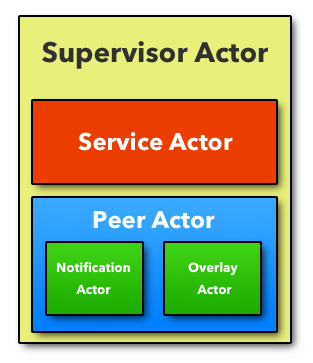
\includegraphics[width=4cm]{./FIGS/these_supervisor.png}

   \hspace*{0.5cm}
	\vspace*{.4cm}
		\caption{The Peer Actor Model}
		{\small The Supervisor actor monitors all the actors it encapsulates while the Peer actor acts as an interface between the services and the overlay.}
\label{fig:supervisor}
   \end{minipage}
\hspace*{0.6cm}
   \begin{minipage}[c]{.55\linewidth}
   	\centering 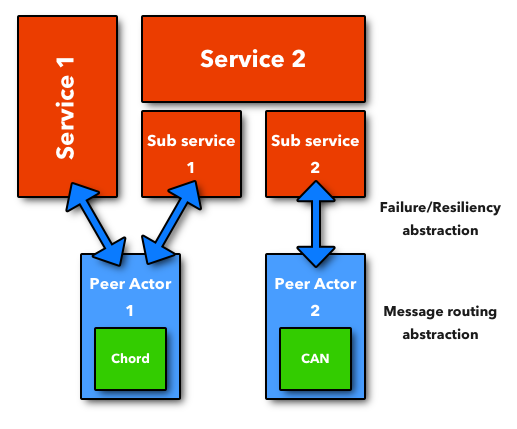
\includegraphics[width=6.5cm]{./FIGS/these_service_peer_archi_legend.png}
	\vspace*{-0.25cm}
		\caption{A Peer Actor Instantiation}
		\label{fig:peeractor} 
{\small The first service relies on a \emph{Peer Actor} implementing a Chord
overlay while the second service uses an additional \emph{PeerActor} implementing a CAN structure.}
  \end{minipage} \hfill
\end{figure}

By such a mean, higher-level services can take the advantage of the advanced
communication layers without dealing with the burden of managing the different
overlays. As an example, when a node disappears, all services that
have been registered as dependent on such an event are notified. 
Service actors can thus react accordingly to the behavior that has been specified. 
%
%Finally, to ensure the reliable execution of the different actors, each one is supervised by a parent entitled 
%the {Supervisor Actor} (see Figure \ref{fig:SupervisorActor}).
%
%
% we consider that at this scale, failures are the norm
%rather than the exception, so we decided that each actor will be monitored
%by a \emph{Supervisor actor}. \discovery services are under the supervision of the
%\
%
%: an actor may crash for a variety of reasons
% we decided that each of the system's actors will be
%supervised by a parent actor called \emph{Supervisor actor} (figure 
%\ref{fig:SupervisorActor}): an actor may crash for a variety of reasons
%(network disruption, byzantine failure, etc.) and it is normal to consider that
%different kind of failures can lead to different reactions of the system. These 
%reactions will be decided by the \emph{Supervisor actor}: reboot of the actor,
%escalation of the error, etc.

Regarding the design and the implementation of the \discovery system, each
service is executed inside its own actor and communicates by
exchanging messages with the other ones. This ensures that each
service is isolated from the others : When a service crashes and needs to be
restarted, the execution of other services is not affected. 
% Besides, each service will be supervised by a global actor that encapsulates all
% services, ie. the \discovery agent. Each time a service fails, the \discovery
% agent catches and analyzes the failure so that it can decide which operations
% to perform. 
%
As previously mentioned, we consider that at the LUC scale, failures are the norm
rather than the exception, hence we decided that each actor will be monitored
by a \emph{Supervisor Actor} (see Figure~\ref{fig:supervisor}). \discovery services are under the supervision of the \discovery agent: this design makes it possible to precisely define strategy
that will be executed in case of service failures. This will be the way we
introduce self-healing and self-organizing properties to the \discovery system.

This building block has been fully implemented\footnote{Code is available at:
\href{https://github.com/BeyondTheClouds}{\url{https://github.com/BeyondTheClouds}}} by 
leveraging the SCALA/akka\footnote{\href{http://www.akka.io}{\url{http://www.akka.io}}} framework.

As a proof of concept, we are implementing a first high level service in charge
of dynamically scheduling VMs across a LUC infrastructure by leveraging the
DVMS~\cite{quesnel:2012} proposal (see Section \ref{ssec:vem}). The low-level
overlay that is currently implemented, is a robust ring based on the  Chord  algorithm. 

% When a node cannot guarantee the QoS for its
%hosted VMs, it starts an iterative scheduling procedure (ISP) by querying its
%neighbor to find a better placement. If the request cannot be satisfied by the
%neighbor (i.e., there is no viable placement to ensure the QoS of all VMs
%hosted on both reserved nodes), the request is forwarded to the following free
%node that takes part in that ISP.  The `absorption' of a new node is repeated
%until the ISP succeeds.  This approach allows DVMS to consider only a minimal
%number of nodes, thus decreasing the scheduling time without requiring a
%central coordinator.  Moreover, it allows several ISPs to occur independently
%at the same moment throughout the infrastructure.  To prevent deadlocks that
%may occur when all nodes are reserved by active ISPs, a distributed deadlock
%prevention mechanism has been designed. It enables DVMS to merge pairs of
%partitions.  To sum things up, the DVMS proposal has been designed to be fully
%distributed, non-predictive and event-driven by using partial views of the
%system.  Such a mechanism perfectly fits the requirements of a LUC OS.  The
%missing part was to extend DVMS in order to take into account resiliency
%aspects. This is going to be solved as we are implementing the DVMS algorithm
%with the \emph{Peer Actor}. 
%

To validate the behavior, the performance as well as the reliability of our
POC, we rely first on the Simgrid~\cite{Casanova:2008:SGF:1397760.1398183}
toolkit. Simgrid has been recently extended to integrate virtualization abstractions and accurate migration models. 
Simulations enable us to analyze particular situations and get several metrics
that cannot be easily monitored  on a real platform.
Second, results obtained from simulations are then compared to real experiments on the Grid'5000 platform. 
Grid'5000 provides a testbed supporting experiments on various types of
distributed systems (high-performance computing, grids, peer-to-peer systems,
Cloud Computing, and others), on all layers of the software stack. The core
testbed currently comprises 10 sites geographically spread across France. 
For the Discovery purpose, we developped a set of scripts that enables to deploy in a \emph{one-click} fashion a large number of VMs throughout 
the whole infrastructure\cite{flauncher}. By deploying our POC on each node and by
leveraging the VM deployment scripts, we can evaluate real scenario usages by conducting specific workloads in the different VMs. 
The validation of this first POC is almost completed. 
The resulting system will be the first to provide reactive,
reliable and scalable
reconfiguration mechanisms of virtual machines in a fully distributed and
autonomous way. This new result will pave the way for a complete proposal of
the \discovery system. 




%\input{implementation}
%\input{evaluation}
%
Cloud Computing has entered our everyday life at a very high speed and huge scale. From classic high performance computing simulations to the management of huge amounts of data coming from mobile devices and sensors, its impact can no longer be minimized. While a lot of progress has already been made in Cloud technologies, there are several concerns that limit the complete adoption of the Cloud Computing paradigm.

In a previous report~\cite{lebre:hal-00854204}, we outlined that, in addition to these concerns, the current model of UC is limited by intrinsic issues. Instead of following the current trend by trying to cope with existing platforms and network interfaces, we proposed to take a different direction by promoting the design of a system that will be efficient and sustainable at the same time, putting knowledge and intelligence directly into the network backbone itself. The innovative approach we introduced will definitely tackle and go beyond Cloud Computing limitations. Our objective is to pave the way for a new generation of Utility Computing that better matches the Internet structure by means of advanced operating mechanisms. By offering the possibility to tightly couple UC servers and network backbones throughout distinct sites and operate them remotely, the LUC OS technology may lead to major changes in the design of UC infrastructures as well as in their environmental impact. The internal mechanisms of the LUC OS should be topology dependent and resources efficient. The natural distribution of the nodes through the different points of presence should be an advantage, which allows to process a request according to its scale: Local requests should be computed locally, while large computations should benefit from a large number of nodes.

The first step toward this highly distributed Cloud infrastructure taking into account locality and network distance is the scheduling of VMs taking into account locality. Thus is this paper, we presented our first building block of our distributed Cloud infrastructure that consists in using P2P algorithms and a vivaldi overlay connected to DVMS, an efficient and flexible VMs scheduler. Our first experiments over Grid'5000 show that, connecting 4 differents sites and scheduling VMs over them, we can gain up to 66\% of inter-sites operations. 

Our future work will consist in ... 

%\bibliographystyle{abbrv}
%\bibliography{refs}

%\appendices
%%%%%%%%%%%%%%%%%%%%%% appendix.tex %%%%%%%%%%%%%%%%%%%%%%%%%%%%%%%%%
%
% sample appendix
%
% Use this file as a template for your own input.
%
%%%%%%%%%%%%%%%%%%%%%%%% Springer-Verlag %%%%%%%%%%%%%%%%%%%%%%%%%%

\chapter{Chapter Heading}
\label{introA} % Always give a unique label
% use \chaptermark{}
% to alter or adjust the chapter heading in the running head

Use the template \emph{appendix.tex} together with the Springer document class SVMono (monograph-type books) or SVMult (edited books) to style appendix of your book in the Springer layout.


\section{Section Heading}
\label{sec:A1}
% Always give a unique label
% and use \ref{<label>} for cross-references
% and \cite{<label>} for bibliographic references
% use \sectionmark{}
% to alter or adjust the section heading in the running head
Instead of simply listing headings of different levels we recommend to let every heading be followed by at least a short passage of text. Further on please use the \LaTeX\ automatism for all your cross-references and citations.


\subsection{Subsection Heading}
\label{sec:A2}
Instead of simply listing headings of different levels we recommend to let every heading be followed by at least a short passage of text. Further on please use the \LaTeX\ automatism for all your cross-references and citations as has already been described in Sect.~\ref{sec:A1}.

For multiline equations we recommend to use the \verb|eqnarray| environment.
\begin{eqnarray}
\vec{a}\times\vec{b}=\vec{c} \nonumber\\
\vec{a}\times\vec{b}=\vec{c}
\label{eq:A01}
\end{eqnarray}

\subsubsection{Subsubsection Heading}
Instead of simply listing headings of different levels we recommend to let every heading be followed by at least a short passage of text. Further on please use the \LaTeX\ automatism for all your cross-references and citations as has already been described in Sect.~\ref{sec:A2}.

Please note that the first line of text that follows a heading is not indented, whereas the first lines of all subsequent paragraphs are.

% For figures use
%
\begin{figure}[t]
\sidecaption[t]
% Use the relevant command for your figure-insertion program
% to insert the figure file.
% For example, with the graphicx style use
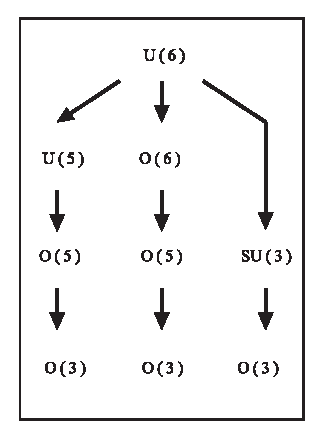
\includegraphics[scale=.65]{figure}
%
% If no graphics program available, insert a blank space i.e. use
%\picplace{5cm}{2cm} % Give the correct figure height and width in cm
%
\caption{Please write your figure caption here}
\label{fig:A1}       % Give a unique label
\end{figure}

% For tables use
%
\begin{table}
\caption{Please write your table caption here}
\label{tab:A1}       % Give a unique label
%
% Follow this input for your own table layout
%
\begin{tabular}{p{2cm}p{2.4cm}p{2cm}p{4.9cm}}
\hline\noalign{\smallskip}
Classes & Subclass & Length & Action Mechanism  \\
\noalign{\smallskip}\hline\noalign{\smallskip}
Translation & mRNA$^a$  & 22 (19--25) & Translation repression, mRNA cleavage\\
Translation & mRNA cleavage & 21 & mRNA cleavage\\
Translation & mRNA  & 21--22 & mRNA cleavage\\
Translation & mRNA  & 24--26 & Histone and DNA Modification\\
\noalign{\smallskip}\hline\noalign{\smallskip}
\end{tabular}
$^a$ Table foot note (with superscript)
\end{table}
%


\subsubsection{Acknowledgments.}
Experiments presented in this paper were carried out using the Grid'5000
experimental testbed, being developed under the INRIA ALADDIN development
 action with support from CNRS, RENATER and several Universities as well as
  other funding bodies (see https://www.grid5000.fr).

\bibliographystyle{llncs2e/splncs03}
\bibliography{main}

\end{document}
